\documentclass[12pt,a4paper]{article}

\usepackage[a4paper,margin=1in]{geometry}
\usepackage{graphicx}
\usepackage{booktabs}
\usepackage{amsmath,amssymb}
\usepackage{float}
\usepackage{hyperref}
\usepackage{xcolor}
\usepackage{listings}
\usepackage{enumitem}
\usepackage{fancyhdr}
\usepackage{longtable}

\hypersetup{colorlinks=true,linkcolor=blue,urlcolor=blue}

\pagestyle{fancy}
\fancyhf{}
\lhead{ICS1512}
\rhead{Machine Learning Algorithms Laboratory}
\cfoot{\thepage}

\lstset{
language=Python,
basicstyle=\ttfamily\small,
numbers=left,
frame=single,
breaklines=true,
showstringspaces=false
}

\begin{document}

\begin{tabular}{|p{4cm}|p{11cm}|}
\hline
Experiment No. & 5 \\ \hline
Experiment Title & Breast Cancer Classification using Decision Tree and Random Forest
\footnote{\textbf{GitHub Repository: }\url{https://github.com/username/repository}}\\ \hline
Student Name & Preethi D \\ \hline
Register Number & 3122247001046 \\ \hline
Faculty & Dr. Poreddy Ajay Kumar Reddy \\ \hline
Submission Date & 15.08.2026 \\ \hline
\end{tabular}

\section{Objective}
To classify breast tumours as malignant or benign using a Decision Tree classifier and a Random Forest ensemble, and to compare their performance after hyperparameter tuning using accuracy, precision, recall, F1-score, and ROC-AUC.

\section{Problem Statement}
Given the Breast Cancer Wisconsin (Diagnostic) dataset, where each sample is described by 30 numeric features computed from digitized images of a breast mass (radius, texture, perimeter, area, smoothness, etc.), the objective is to predict whether the tumour is malignant or benign. Input: 30 numeric features per sample. Output: binary class label (malignant/benign). Both a single Decision Tree and a Random Forest ensemble are trained, tuned via GridSearchCV, and compared.

\section{Dataset Description}
\begin{longtable}{|p{6cm}|p{8cm}|}
\hline
Dataset Name & Breast Cancer Wisconsin (Diagnostic) \\ \hline
Dataset Source & Scikit-learn built-in dataset (\texttt{sklearn.datasets.load\_breast\_cancer}), originally from UCI Machine Learning Repository \\ \hline
Number of Samples & 569 \\ \hline
Number of Features & 30 numeric features (mean, standard-error, and worst-case measurements of cell-nuclei characteristics) \\ \hline
Number of Classes & 2 (0 = malignant, 1 = benign) \\ \hline
Missing Values & 0 \\ \hline
Train-Test Split & 80\% train / 20\% test (stratified), giving 455 training and 114 test samples \\ \hline
\end{longtable}

\section{Exploratory Data Analysis}

\begin{figure}[H]
\centering
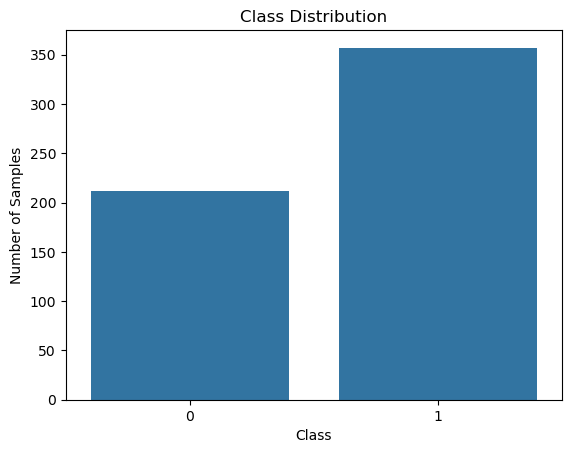
\includegraphics[width=0.55\linewidth]{images/class_distribution.png}
\caption{Class distribution of the Breast Cancer dataset}
\end{figure}
\textbf{Inference:} The dataset is moderately imbalanced, with 357 benign samples versus 212 malignant samples (roughly a 5:3 ratio). This imbalance is mild enough that accuracy remains a reasonably informative metric, but precision, recall, and F1-score were still tracked separately to ensure the minority (malignant) class is not being predicted poorly, since misclassifying a malignant tumour as benign is the more costly error clinically.

\begin{figure}[H]
\centering
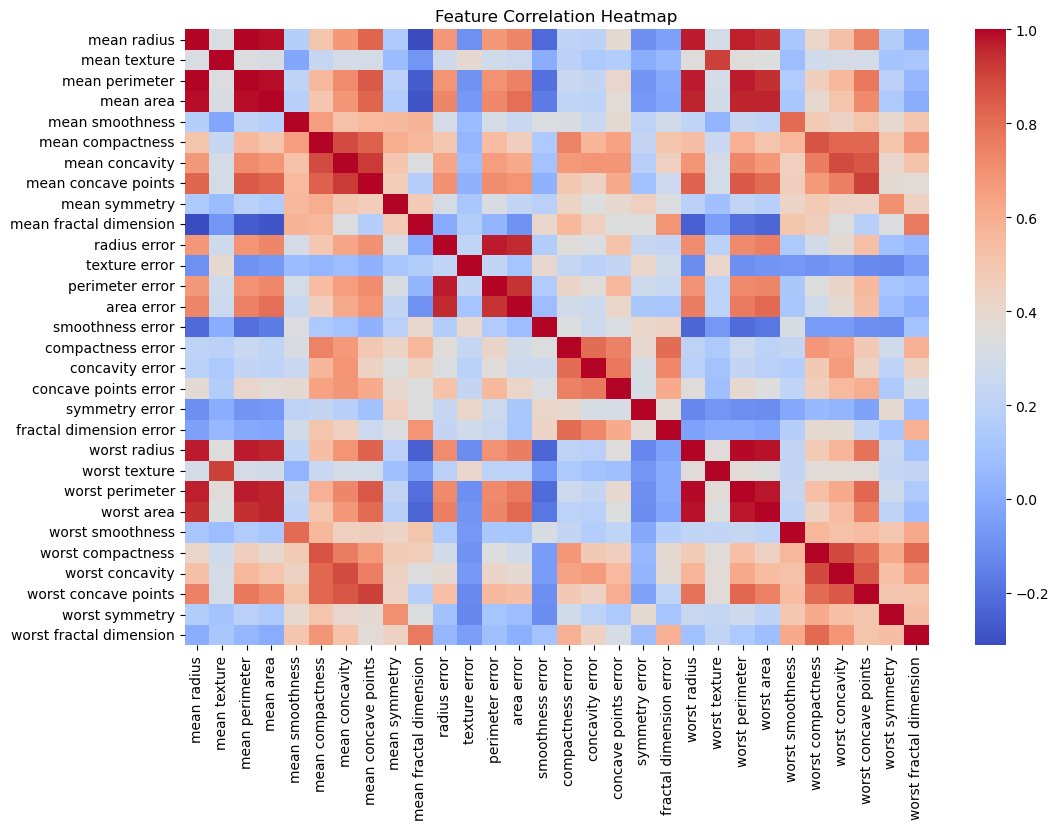
\includegraphics[width=0.75\linewidth]{images/corr_heatmap.png}
\caption{Correlation heatmap of all 30 features}
\end{figure}
\textbf{Inference:} Many features are very strongly correlated with each other, particularly the "mean", "standard error", and "worst" versions of the same underlying measurement (e.g.\ radius, perimeter, and area), since these are mathematically related quantities computed from the same cell-nuclei outlines. This high multicollinearity suggests that tree-based models, which are not sensitive to correlated features the way linear models are, are a good fit for this dataset, and that feature-importance rankings should be interpreted with some caution given the redundancy.

\section{Data Preprocessing}

\begin{itemize}
\item \textbf{Missing value handling:} None required -- the dataset has zero missing values across all 30 features.
\item \textbf{Encoding:} Not required; the target is already numeric (0 = malignant, 1 = benign) and all features are continuous numeric measurements.
\item \textbf{Feature scaling:} Not applied, since both Decision Tree and Random Forest are tree-based models that split on feature thresholds and are invariant to monotonic feature scaling.
\item \textbf{Train-test split:} An 80/20 stratified split was used (\texttt{train\_test\_split} with \texttt{stratify=y}, \texttt{random\_state=42}), giving 455 training samples and 114 test samples while preserving the original class ratio.
\item \textbf{Feature engineering:} None -- all 30 original features were used directly as model inputs.
\end{itemize}

\section{Machine Learning Algorithm}

\textbf{Decision Tree:}
\begin{itemize}
\item \textbf{Working principle:} A Decision Tree recursively splits the feature space into regions by choosing, at each node, the feature and threshold that best separates the classes according to an impurity measure, continuing until a stopping criterion (max depth, minimum samples per leaf, etc.) is reached.
\item \textbf{Mathematical formulation:} Splits are chosen to minimize impurity, e.g.\ the Gini index $G = 1-\sum_{k}p_k^2$ or entropy $H = -\sum_{k}p_k\log_2 p_k$, where $p_k$ is the proportion of class $k$ samples in a node; the split maximizing the impurity reduction (information gain) is selected at each step.
\item \textbf{Advantages:} Easy to interpret and visualize, requires no feature scaling, and can naturally capture non-linear relationships and feature interactions.
\item \textbf{Limitations:} Prone to overfitting if grown too deep (a single unconstrained tree can memorize the training data), and can be unstable -- small changes in the data can produce a very different tree structure.
\end{itemize}

\textbf{Random Forest:}
\begin{itemize}
\item \textbf{Working principle:} Random Forest builds an ensemble (bag) of many Decision Trees, each trained on a bootstrap-resampled subset of the training data and considering only a random subset of features at each split, then aggregates their predictions by majority vote (classification).
\item \textbf{Mathematical formulation:} For $T$ trees, the ensemble prediction is $\hat{y} = \text{mode}\{h_1(x), h_2(x), \dots, h_T(x)\}$, where each $h_t$ is trained on a bootstrap sample $D_t$ drawn with replacement from the training set, and each split considers a random subset of \texttt{max\_features} candidate features.
\item \textbf{Advantages:} Averaging over many de-correlated trees substantially reduces the variance/overfitting seen in a single Decision Tree, generally improves accuracy and robustness, and provides a natural measure of feature importance.
\item \textbf{Limitations:} Less interpretable than a single tree (it is effectively a "black box" ensemble), more computationally expensive to train and tune due to the larger hyperparameter space, and can still overfit if trees are allowed to grow fully deep without any regularization.
\end{itemize}

\section{Experimental Setup}
\begin{tabular}{ll}
\toprule
Python Version & \\
Scikit-Learn Version & \\
IDE & Jupyter Notebook \\
Operating System & Windows \\
Hardware & \\
\bottomrule
\end{tabular}

\section{Hyperparameter Selection}

\textbf{GridSearchCV -- Decision Tree (5-fold, scoring=accuracy):}
\begin{tabular}{ll}
\toprule
Parameter & Value / Search Space\\
\midrule
criterion searched & gini, entropy \\
max\_depth searched & 3, 5, 7, None \\
min\_samples\_split searched & 2, 5, 10 \\
min\_samples\_leaf searched & 1, 2, 4 \\
\textbf{Best criterion} & \textbf{gini} \\
\textbf{Best max\_depth} & \textbf{5} \\
\textbf{Best min\_samples\_leaf} & \textbf{1} \\
\textbf{Best min\_samples\_split} & \textbf{5} \\
Best CV accuracy & 0.9385 \\
Best CV F1-score (separate search) & 0.9518 \\
\bottomrule
\end{tabular}

\vspace{0.3cm}
\textbf{GridSearchCV -- Random Forest (5-fold, scoring=accuracy):}
\begin{tabular}{ll}
\toprule
Parameter & Value / Search Space\\
\midrule
n\_estimators searched & 50, 100 \\
max\_depth searched & 3, 5, 7, None \\
max\_features searched & sqrt, log2 \\
bootstrap searched & True, False \\
\textbf{Best n\_estimators} & \textbf{100} \\
\textbf{Best max\_depth} & \textbf{None} \\
\textbf{Best max\_features} & \textbf{log2} \\
\textbf{Best bootstrap} & \textbf{False} \\
Best CV accuracy & 0.9692 \\
\bottomrule
\end{tabular}

\section{Results}

\textbf{Test set (114 samples), tuned models:}
\begin{longtable}{lccccc}
\toprule
Model & Accuracy & Precision & Recall & F1-score & AUC\\
\midrule
\endhead
Decision Tree & 92.11\% & 95.65\% & 91.67\% & 93.62\% & 0.9163 \\
Random Forest & \textbf{95.61\%} & \textbf{95.89\%} & \textbf{97.22\%} & \textbf{96.55\%} & \textbf{0.9944} \\
\bottomrule
\end{longtable}

\textbf{5-Fold Stratified Cross-Validation (training set, tuned models):}
\begin{longtable}{lcccccc}
\toprule
Model & Fold 1 & Fold 2 & Fold 3 & Fold 4 & Fold 5 & Average\\
\midrule
\endhead
Decision Tree & 94.51\% & 92.31\% & 91.21\% & 92.31\% & 89.01\% & 91.87\% \\
Random Forest & 95.60\% & 98.90\% & 93.41\% & 94.51\% & 97.80\% & \textbf{96.04\%} \\
\bottomrule
\end{longtable}

\section{Result Visualization}

\begin{figure}[H]
\centering
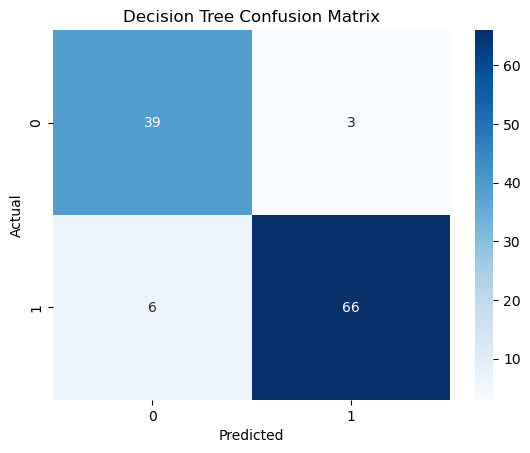
\includegraphics[width=0.45\linewidth]{images/cm_decision_tree.png}
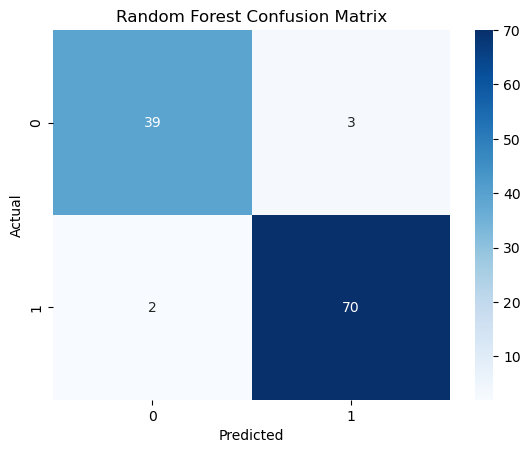
\includegraphics[width=0.45\linewidth]{images/cm_random_forest.png}
\caption{Confusion matrices: Decision Tree (left) and Random Forest (right)}
\end{figure}
\textbf{Inference:} Random Forest makes noticeably fewer errors than the Decision Tree overall, and in particular produces fewer false negatives (malignant cases misclassified as benign) -- the more clinically dangerous type of error. This is reflected in Random Forest's higher recall (97.22\% vs.\ 91.67\%), showing the ensemble is substantially better at catching true malignant cases.

\begin{figure}[H]
\centering
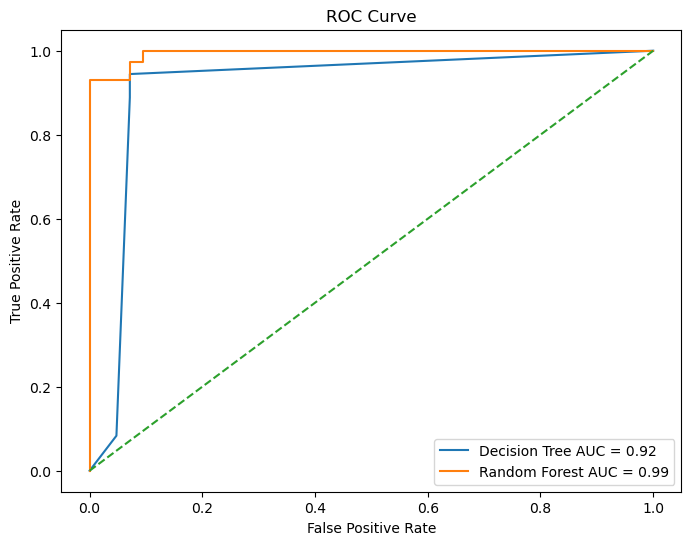
\includegraphics[width=0.65\linewidth]{images/roc_curve.png}
\caption{ROC curves for Decision Tree and Random Forest}
\end{figure}
\textbf{Inference:} The Random Forest ROC curve hugs the top-left corner far more closely than the Decision Tree's, giving a near-perfect AUC of 0.994 compared to 0.916 for the single tree. This large AUC gap shows that Random Forest's predicted probabilities are much better calibrated and more reliably rank malignant cases above benign ones across all classification thresholds, not just the default 0.5 cutoff.

\section{Discussion}

Random Forest clearly outperformed the single Decision Tree across every metric measured -- accuracy, precision, recall, F1-score, and especially AUC (0.994 vs.\ 0.916) -- which is the expected and well-documented benefit of ensembling many de-correlated trees to reduce variance. The gap is particularly pronounced in cross-validation, where Random Forest's average accuracy (96.04\%) was both higher and far more stable across folds (ranging 93.4--98.9\%) than the Decision Tree's (91.87\% average, ranging 89.0--94.5\%), confirming that the ensemble generalizes more reliably rather than just performing well on one lucky split. From a clinical-risk perspective, Random Forest's substantially higher recall (97.22\% vs.\ 91.67\%) is especially important, since it means fewer malignant tumours are missed. The main trade-off is interpretability: the tuned Random Forest with \texttt{max\_depth=None} and \texttt{bootstrap=False} is effectively a black box compared to the single, visualizable Decision Tree, and further work could explore feature-importance analysis to partially recover interpretability while keeping the ensemble's accuracy advantage.

\section{Conclusion}

This experiment implemented and compared a Decision Tree and a Random Forest classifier for malignant/benign breast tumour classification on the Breast Cancer Wisconsin dataset. After hyperparameter tuning via GridSearchCV, Random Forest (100 trees, no bootstrap, \texttt{log2} max features) clearly outperformed the single Decision Tree, achieving 95.61\% test accuracy and a near-perfect AUC of 0.994, confirming the practical benefit of ensemble methods over a single tree for this classification task.

\section{References}
\begin{enumerate}
\item W. H. Wolberg, W. N. Street, and O. L. Mangasarian, ``Breast Cancer Wisconsin (Diagnostic) Data Set,'' UCI Machine Learning Repository, 1995.
\item F. Pedregosa \textit{et al.}, ``Scikit-learn: Machine Learning in Python,'' \textit{Journal of Machine Learning Research}, vol. 12, pp. 2825--2830, 2011.
\item L. Breiman, ``Random Forests,'' \textit{Machine Learning}, vol. 45, no. 1, pp. 5--32, 2001.
\item L. Breiman, J. H. Friedman, R. A. Olshen, and C. J. Stone, \textit{Classification and Regression Trees}. Wadsworth, 1984.
\end{enumerate}

\end{document}
